\documentclass[a4paper,twoside,12pt,chapterprefix=false]{scrbook}

\usepackage{amsmath,amssymb,amsthm}
\usepackage{longtable} % tables over several pages
\usepackage[font={small,sl},hang,labelfont=bf]{caption} % configure captions
%\usepackage{captcont} % continue sufigures over several pages
\usepackage{booktabs} % publication quality tables for LaTeX
%\usepackage{showkeys} % shows the labels above the references for easier development

\usepackage{acronym}
\usepackage{subfig}

\ifpdfoutput{%
	\usepackage[pdftex]{graphicx}
	\usepackage[]{pdfpages} %for including full pdf pages
}{%
	\usepackage{graphicx}
}
\usepackage{rotating} % rotate figures

\usepackage{scrpage2}
\KOMAoptions{headinclude}

% Font packages:
\usepackage{times}
\usepackage{helvet}   % sets sans serif font
\usepackage[utf8]{inputenc}

% Listings:
\usepackage{listings}

%PDF hyperref config
\ifpdfoutput{%
	\usepackage[pdftex,
		bookmarks,
		bookmarksopen=true,
		bookmarksnumbered=true,
		pdfauthor={My Name},
		pdftitle={Thesis Title},
		colorlinks,
		linkcolor=black,
		citecolor=black,
		filecolor=black,
		urlcolor=black,
		anchorcolor=black,
		menucolor=black,
		breaklinks=true,
		pageanchor=true,
		plainpages=false,
		pdfpagelabels=true]{hyperref}
}{}

\ifpdfoutput{%
	\pdfcompresslevel=9
	\pdfoutput=1
	\DeclareGraphicsExtensions{.pdf,.png,.eps}
}{}

\bibliographystyle{apalike}

% Uncomment the chapter / section you are working on.
%
%\includeonly{figures}
%\includeonly{tables}
%\includeonly{data-analysis}
%\includeonly{conclusion}
%\includeonly{apx-sample-appendix}

%\pagestyle{useheadings}

% A4
%
\topmargin -0.5in
\textheight 9.3in
\textwidth 6.3in
\oddsidemargin 0.18in
\evensidemargin -0.22in
\parskip 0.1in
\parindent 0in

\renewcommand{\arraystretch}{1.5}
\renewcommand{\baselinestretch}{1}


\begin{document}

%  Terminates current page and paragraph, makes sure next page starts on
%  an odd-number, and generates a completely blank page, without page markers,
%  if necessary.
\newcommand{\clearemptydoublepage}{\newpage{\pagestyle{empty}\cleardoublepage}}



\acrodef{ar}[\textsc{ar}]{Augmented Reality}
\acrodef{vr}[\textsc{vr}]{Virtual Reality}
\acrodef{hmd}[\textsc{hmd}]{Head-Mounted Display}
\acrodef{nes}[\textsc{nes}]{Nintendo Entertainment System}
\acrodef{cmos}[\textsc{cmos}]{Complementary Metal-Oxide-Semiconductor}
\acrodef{ai}[\textsc{ai}]{Artificial Intelligence}
\acrodef{its}[\textsc{its}]{Intelligent Tutoring System}
\acrodef{rpm}[\textsc{rpm}]{revolutions per minute}
\acrodef{zpdes}[\textsc{zpdes}]{Zone of Proximal Development and Empirical Success}
\acrodef{zpd}[\textsc{zpd}]{Zone of Proximal Development}
\acrodef{lod}[\textsc{lod}]{Level of Detail}
\acrodef{dof}[\textsc{dof}]{Degrees of Freedom}
\acrodef{fps}[\textsc{fps}]{Frames per Second}
\acrodef{satnav}[satnav]{Satellite Navigation System}

\newcommand{\refsec}[1]{Section~\ref{sec:#1}}
\newcommand{\refeq}[1]{Eq.~(\ref{eq:#1})}
\newcommand{\reffig}[1]{Figure~\ref{fig:#1}}
\newcommand{\reftab}[1]{Table~\ref{tab:#1}}
\newcommand{\refalg}[1]{Alg.~(\ref{alg:#1})}


\newcommand{\todo}[1]{\textcolor{red}{TODO: #1}}

%% Define leading chapter pages
%
\input{studchapter}
\newpagestyle{mychapterpagestyle}{{\protect\mychpstyleintl}{\protect\mychpstyleintl}}{}
\newpagestyle{myappendixpagestyle}{{\protect\mychpstyleintl}{\protect\mychpstyleintl}}{}
%%


\hypersetup{pageanchor=false} % disabling anchors for title page to avoid warning

%% Replace this by your own design of a title page
%
%\title{Thesis Title}
%\author{My Name}
%\date{September 2042}
%\maketitle
%\clearemptydoublepage
% --- selfmade version ----
\begin{titlepage}
	\topmargin 1.0cm
	\oddsidemargin 0.0cm
	\evensidemargin 0.0cm
	%\textwidth 6.5in
	\centering
	\Huge
	\vspace{3.0cm}
	\textbf{\textsf{Thesis Title}} \\[2.0cm]


	\todo{Put nice teaser image here}


	%\includegraphics*[width=0.4\textwidth]{figures/titlefigure} \\[4.0cm]
	\vspace{5.0cm}
	\sffamily
	\Large
	My Name
	\\[0.8cm]
	\large
	Master Thesis
	\\
	September 2042
	\\[1.3cm]
	Dr. Stéphane Magnenat, Dr. Fabio Zünd\\
	Prof. Dr. Robert W. Sumner
	\vfill
	\includegraphics*[width=0.3\textwidth]{figures/eth_logo_lang_pos} \hfill
	\includegraphics*[width=0.3\textwidth]{figures/GTC_ColorBlack}
	\vspace{3.4cm}
\end{titlepage}
\clearemptydoublepage
%%

\hypersetup{pageanchor=true}
\pagenumbering{roman}
\setcounter{page}{1}

\chapter*{Abstract}
This thesis addresses the development of a novel sample thesis. We analyze the requirements of a general template, as it can be used with the \LaTeX\ text processing system. (And so on\dots) The abstract should not exceed half a page in size!



%include acknowledgment here:
\chapter*{Acknowledgements}
\input{tex/acknowledgments}

\tableofcontents
\cleardoublepage

\addcontentsline{toc}{chapter}{List of Figures}
\listoffigures
\cleardoublepage

\addcontentsline{toc}{chapter}{List of Tables}
\listoftables
\cleardoublepage

\pagenumbering{arabic}
\renewcommand*{\chapterpagestyle}{mychapterpagestyle}
\renewcommand*{\chapterformat}{} % show chapter titles only (no numbers)
% \setchapterpreamble[o]{...}  unfortunately does not move the \chapter output downwards

% ---- MAIN PART ----

% set counter to n-1:
\setcounter{chapter}{0}

\chapter{Introduction}\label{sec:introduction}


Use acronyms: Novel technology, such as \ac{ar} and \ac{vr}, has ...

\todo{These are todo texts.}

Use references like this: This text is described in more detail in \refsec{introduction} but not in \refsec{relatedwork}. Finally, \reftab{mytable} contains valuable results. For figures with multiple images, you can use \reffig{twofigures} \subref{fig:twofigures:IgeaNarrowBand}.
% set counter to n-1:
\setcounter{chapter}{1}

\chapter{Related Work}\label{sec:relatedwork}


Sample references are~\cite{Zwicker04Perspective} and~\cite{Altman89QuaternionScandal}. 
Lorem ipsum dolor sit amet, consectetuer adipiscing elit, sed diam nonummy nibh euismod tincidunt ut laoreet dolore magna aliquam erat volutpat. Ut wisi enim ad minim veniam, quis nostrud exerci tation ullamcorper suscipit lobortis nisl ut aliquip ex ea commodo consequat. Duis autem vel eum iriure dolor in hendrerit in vulputate velit esse molestie consequat, vel illum dolore eu feugiat nulla facilisis at vero et accumsan et iusto odio dignissim qui.


\section{Appearance Modeling}


Lorem ipsum dolor sit amet, consectetuer adipiscing elit, sed diam nonummy nibh euismod tincidunt ut laoreet dolore magna aliquam erat volutpat. Ut wisi enim ad minim veniam, quis nostrud exerci tation ullamcorper suscipit lobortis nisl ut aliquip ex ea commodo consequat. Duis autem vel eum iriure dolor in hendrerit in vulputate velit esse molestie consequat, vel illum dolore eu feugiat nulla facilisis at vero et accumsan et iusto odio dignissim qui.

\subsection{Taxonomy}

Lorem ipsum dolor sit amet, consectetuer adipiscing elit, sed diam nonummy nibh euismod tincidunt ut laoreet dolore magna aliquam erat volutpat. Ut wisi enim ad minim veniam, quis nostrud exerci tation ullamcorper suscipit lobortis nisl ut aliquip ex ea commodo consequat. Duis autem vel eum iriure dolor in hendrerit in vulputate velit esse molestie consequat, vel illum dolore eu feugiat nulla facilisis at vero et accumsan et iusto odio dignissim qui.

\chapter{Your Central Work}

Always put text between section titles.

\section{Section}

\begin{lstlisting}[mathescape]
$i$ := $0$;
$j$ := $\frac{n}{2}$;
while $i$ $\leq$ $\frac{n}{2}$ and $j$ $\geq$ $0$ do
	if $l_x$[$i$] = b or $l_y$[$j$] = b then
		return true;
	end
	if $l_x$[$i$] + $l_y$[$j$] < b then
		$i$ := $i$ + $1$;
	else if $l_x$[$i$] + $l_y$[$j$] > b then
		$j$ := $j$ - $1$;
	else
		return true;
	end
end
return false;
\end{lstlisting}


\subsection{Another Subsection}

\begin{table}
    \centering
		\caption[Flammkuchenteig]{Flammkuchenteig. The ingredients have to be carefully chosen.\label{tab:mytable}}
    \begin{tabular}{|l|p{0.4\linewidth}|}
    \hline
    \emph{Quant.} & \emph{Ingredient}\\
    \hline
		200g &Wei{\ss}mehl\\
		1/4  &Packung Frischhefe\\
		4EL  &lauwarme Milch\\
		4EL  &Öl\\
		1TL  &Zucker\\
		1TL  &Salz\\
		&lauwarmes Wasser\\
    \hline
    \end{tabular}    
\end{table}

\subsection{More Subsections}


\begin{figure}[htb]
     \centering
     \subfloat[][Caption first]{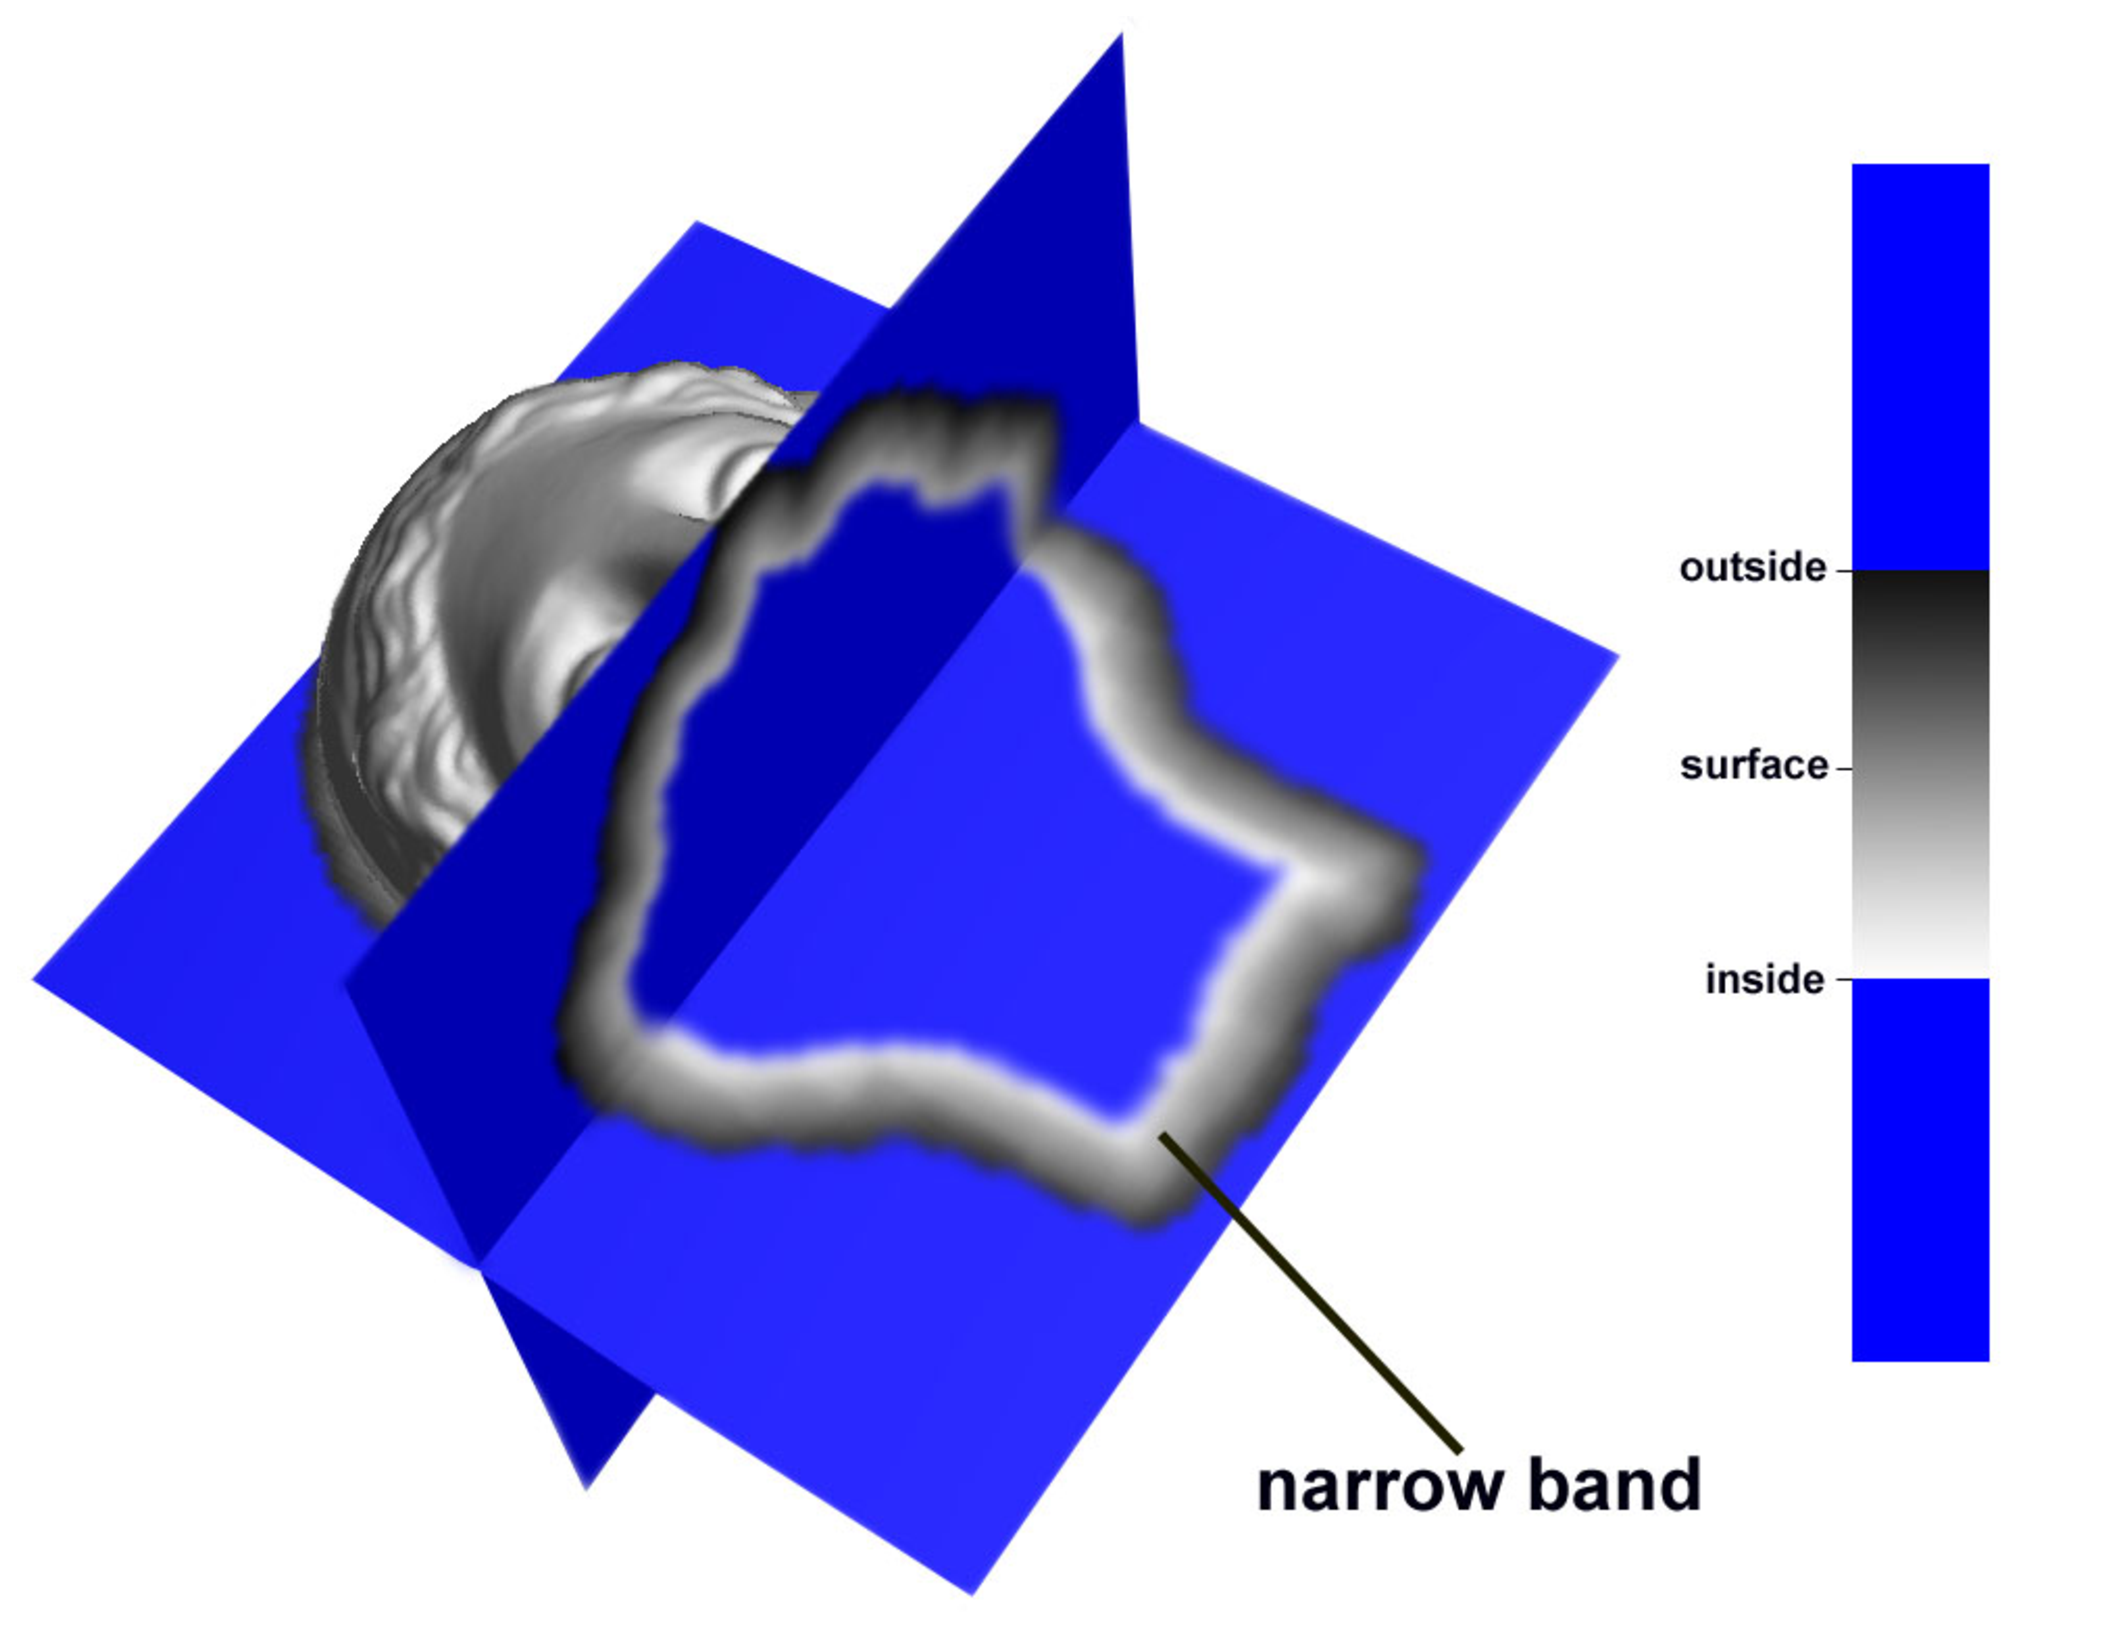
\includegraphics[width=0.45\textwidth]{figures/IgeaNarrowBand}\label{fig:twofigures:IgeaNarrowBand}}
     \subfloat[][Caption first]{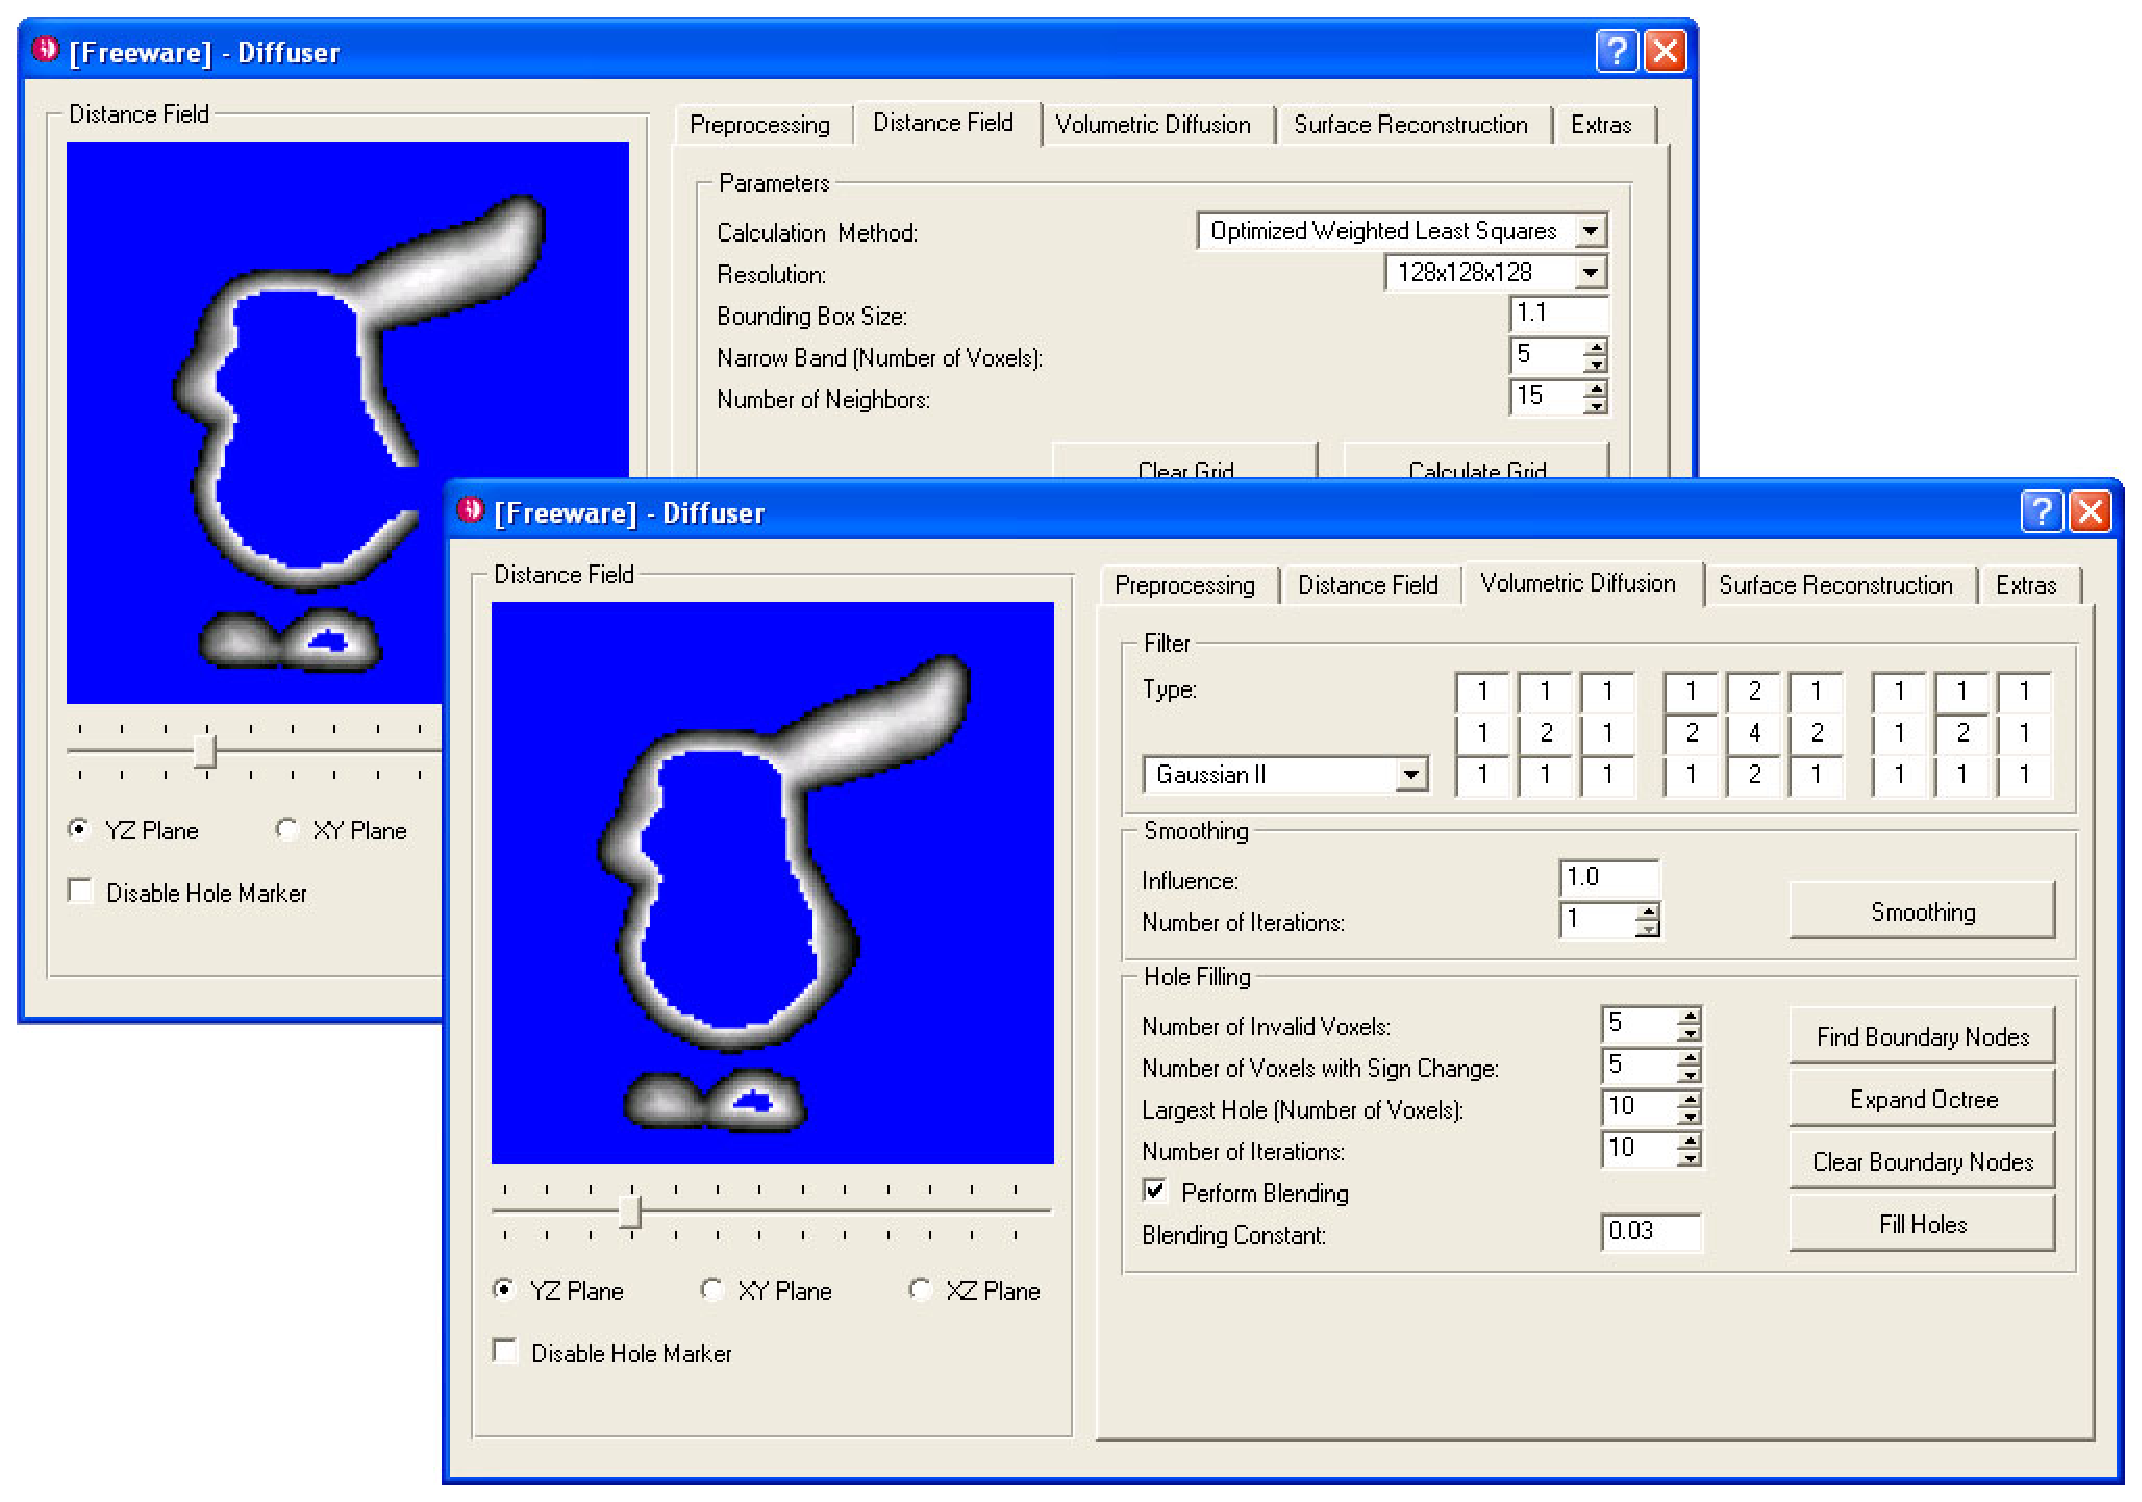
\includegraphics[width=0.45\textwidth]{figures/voldiff_ui}\label{fig:twofigures:voldiff_ui}}
     \caption{Comparison of steady state results. \protect\subref{fig:twofigures:IgeaNarrowBand} x method and \protect\subref{fig:twofigures:voldiff_ui} y method.}
     \label{fig:twofigures}
\end{figure}


\input{tex/results}
\input{tex/conclusion}


% ---- END MAIN PART ----


\appendix
\clearpage
\renewcommand*{\chapterpagestyle}{myappendixpagestyle}

\input{tex/apx-sample-appendix}

\clearpage
\renewcommand*{\chapterpagestyle}{empty}

%\nocite{*}
\addcontentsline{toc}{chapter}{Bibliography}
\bibliography{graphics}


%include task description here:
\cleardoublepage
\todo{put project description here}
%\includegraphics[viewport=3cm 0cm 20cm 27.5cm]{task_description} %better use includepdf below!
%\includepdf{task_description}
\cleardoublepage

%include eigenstaendigkeitserklaerung
\cleardoublepage
\todo{put eigenstaendigkeitserklaerung here}
%\includepdf{asdasdasd}
\cleardoublepage





\end{document}
